\documentclass[12pt]{article}
\usepackage{setspace}
\doublespacing

\usepackage{amsmath}
\usepackage[margin = 1in]{geometry}
\usepackage{graphicx}
\usepackage{booktabs}
\usepackage{natbib}
\usepackage[colorlinks=true, citecolor=blue]{hyperref}

\title{Predicting Diabetes Based on Various Factors Using Decision Trees}
\author{Ashley Merritt\\
    Department of Statistics\\
    University of Connecticut
    }

\begin{document}
\maketitle

\begin{abstract}
This section will be completed once the paper is closer to completion. 
\end{abstract}


\section{Introduction}
\label{sec:intro}
    According to the American Diabetes Association, about 11.3 percent of Americans, or about 37.3 million people, have diabetes.
    Of those 37.3 million people, about 28.7 million were actually diagnosed with diabetes, while the remaining 8.6 million were
    left undiagnosed (\citet{CDC2022Diabetes}). Those left undiagnosed are at risk for even more serious illness if left untreated. 
    Diabetes is a disease where your body does not create enough insulin, or use it properly, in order to get glucose into your cells 
    and use it for energy (\cite{NIH2023Whatis}). Therefore, it is very important that your body has a normal glucose level. In this 
    paper, I will be working to determine the pre-existing factors that can be used in order to predict if a person may have diabetes. 
    Establishing the predictors is very important to me as many of my family members have a long history of suffering from this disease. 
    It is important to better predict this disease to save people from unnecessary suffering. 

    Previously, the prediction of diabetes has been studied using machine learning models. Specifically in Sisodia's paper, it focused
    on the "Prediction of Diabetes using Classification Algorithms", they worked through the topic by producing results using support 
    vector machine, Naive Bayes classifier, and decision tree classifier (\cite{Sisodia2018Prediction}). In this paper, I will be 
    continuing the investigation with a different data set using decision trees.

    In this paper the specific research question that I will be focusing on is: how can we use machine learning models in order to identify 
    individuals that may have already or are at risk at developing diabetes? This will be researched using a data set that contains various 
    metrics on one's health that will be described in the next section of the paper.

    The rest of the paper is organized as follows.
    The data will be presented in Section~\ref{sec:data}.
    The methods are described in Section~\ref{sec:meth}.
    The results are reported in Section~\ref{sec:resu}.
    A discussion concludes in Section~\ref{sec:disc}.

\section{Data}
\label{sec:data}
    In order to study the proposed research question on the topic of diabetes, I searched through many databases in order to find a set 
    that had all of the information I was looking for. After exploration, I found a data set entitled "Healthcare Diabetes Data set" on 
    the website Kaggle. The data set was originally sourced from the National Institute of Diabetes and Digestive and Kidney Diseases. The 
    data encompasses eight different predictors including pregnancies, glucose, blood pressure, skin thickness, insulin, BMI, diabetes 
    pedigree function, and age. In Table~\ref{tab:head_of_data} I will provide the first couple lines of dataset in order to provide
    more information on the dataset.

    \begin{table}[ht]
    \caption{Head of the Dataset}
    \centering
    \resizebox{\textwidth}{!}{%
    \begin{tabular}{rrrrrrrrr}
      \hline
    Pregnancies & Glucose & BloodPressure & SkinThickness & Insulin & BMI & DiabetesPedigreeFunction & Age & Outcome \\ 
      \hline
      6 & 148 &  72 &  35 &   0 & 33.60 & 0.63 &  50 &   1 \\ 
        1 &  85 &  66 &  29 &   0 & 26.60 & 0.35 &  31 &   0 \\ 
        8 & 183 &  64 &   0 &   0 & 23.30 & 0.67 &  32 &   1 \\ 
        1 &  89 &  66 &  23 &  94 & 28.10 & 0.17 &  21 &   0 \\ 
        0 & 137 &  40 &  35 & 168 & 43.10 & 2.29 &  33 &   1 \\ 
        5 & 116 &  74 &   0 &   0 & 25.60 & 0.20 &  30 &   0 \\ 
       \hline
    \end{tabular}%
    } 
    \label{tab:head_of_data}
    \end{table}
    

    The predictors listed above will be represented in my research as the following variables. 'Pregnancies' will provide the number of 
    times an entry has been pregnant. 'Glucose' will provide the plasma glucose concentration over two hours using the results of an oral 
    glucose tolerance test on a entry. 'BloodPressure' gives the diastolic blood pressure in mm Hg of an entry. 'SkinThickness' will 
    provide the triceps skin fold thickness in mm. 'Insulin' will include a test on two hour serum insulin in mu U/ml. 'BMI' will provide a 
    calculation of weight (kg) divided by height ($m^2$). 'DiabetesPedigreeFunction' will provide a genetic score of diabetes. 'Age' will 
    simply be the entry's age at the time of the collection. Following this paragraph, I will provide the link to the dataset that I will 
    be using as well as showing some descriptive statistics in Table~\ref{tab:ds} including the mean, standard deviation, and median.  

Dataset link: \href{https://www.kaggle.com/datasets/nanditapore/healthcare-diabetes}{Healthcare Diabetes}

\begin{table}[ht]
    \caption{Descriptive Statistics of Healthcare Diabetes Dataset}
  \label{tab:ds}
\centering
\begin{tabular}{lrrr}
      \hline
    Variable & Mean & SD & Median \\ 
      \hline
      Pregnancies & 3.74 & 3.32 & 3.00 \\ 
      Glucose & 121.10 & 32.04 & 117.00 \\ 
      BloodPressure & 69.13 & 19.23 & 72.00 \\ 
      SkinThickness & 20.82 & 16.06 & 23.00 \\ 
      Insulin & 80.13 & 112.30 & 37.00 \\ 
      BMI & 32.14 & 8.08 & 32.20 \\ 
      DiabetesPedigreeFunction & 0.47 & 0.33 & 0.38 \\ 
      Age & 33.13 & 11.78 & 29.00 \\ 
       \hline
    \end{tabular}
    \end{table}

\section{Methods}
\label{sec:meth}
    Various methods will be used to complete the statistical analysis necessary for this project. I will begin by exploring basic 
    descriptive statistics to gain an understanding of my data set. I will then begin to create my model for my decision tree by
    splitting the data into a test and training set. The training set will encompass 80 percent of the data whereas the test set will
    only have 20 percent. After creating these two sets we will now be ready to build the model, this will be done by using the rpart
    function in R, where method will be 'class' as this is a binary model. We will then see in Figure~\ref{fig:structure} the structure
    of the decision tree created. Looking at the leftmost path in the decision tree we can see that at the top the outcome was 0 meaning 
    that the patient did not have diabetes 35 percent of the time. Moving down to the next node, we can see that 68 percent of patients with
    glucose level less than 128, did not have diabetes 19 percent of the time. To finish this path, 61 percent of the time if the patient was
    older than 29 years old, then 8 percent of the time the patient had diabetes. The rest of the structure is similar but with different 
    values and predictors.

\begin{figure}[tbp]
  \centering
  \caption{Decision Tree Structure}
  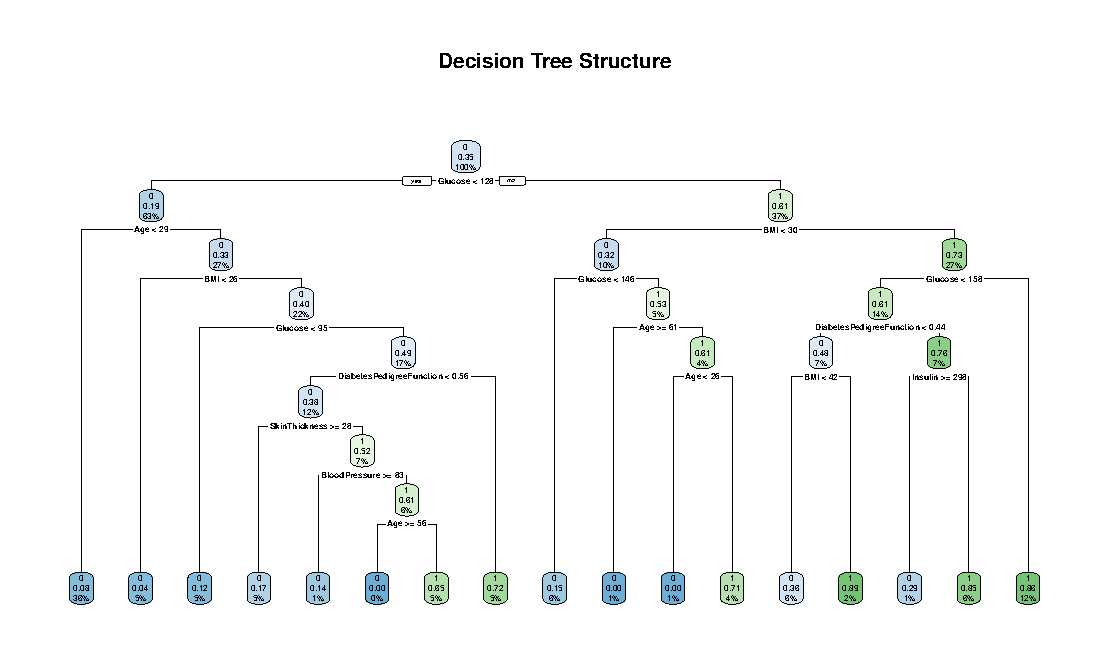
\includegraphics[width=\textwidth]{Decision Tree Structure.pdf}
  \label{fig:structure}
  \end{figure}

\begin{table}[ht]
  \centering
  \caption{Confusion Matrix} 
  \begin{tabular}{rrr}
    \toprule
    & 0 & 1 \\ 
    \midrule
  0 & 318 & 47 \\ 
    1 & 53 & 136 \\ 
    \bottomrule
  \end{tabular}
  \label{tab:conf_matrix}
  \end{table}

\section{Results}
\label{sec:resu}

After completing our methods section, we can now move on to talk about the results of our model. Based on our logistic regression model, 
we now know that all of the predictors in the data set except skin thickness are important in order to predict whether a patient may have 
diabetes or not. With this information medical professionals will be able to ensure proper treatment to patients as they can use these 
predictors in order to tell if a patient may have diabetes even sooner than typical means. The model allows for medical professionals to 
use the model in order to further their research into diabetes and the various precursors.

\section{Discussion}
\label{sec:disc}

Currently, this study is limited as we are set within the bounds of this data set. In future studies we can include more predictors in 
order to see if there are any other factors that could be used to predict diabetes. As well as having an even larger data set in order to 
ensure our accuracy. Other data sets may suggest that certain predictors are not helpful in predicting diabetes that our model did not pick 
up on due to the metrics of our data. 


As this is a paper dealing with sensitive medical data, we have many limitations in order to be ethical as well as respecting patient 
privacy. Based on the data set collected we should be able to ensure patient privacy pretty well as names or any very unique identifiers 
are not listed with each entry. We simply have a ID and age for each entry so we do not have to worry as much for the sake of privacy. In 
terms of our direct models we may have to disregard some assumptions as they may not fit with real world data. If something unexpected 
happens we may have to reconsider the data set used and consider finding a new one. This will be done by a case by case scenario and will 
be investigated thoroughly before making any decisions.

\bibliography{refs}
\bibliographystyle{mcap}

\end{document}

